\section{什么是计算机科学}

计算机科学往往难以定义。这可能是由于在名称中不幸使用了“计算机”一词。正如你可能知道的,计算机科学不仅仅是计算机的研究。虽然计算机作为一个工具在学科中发挥重要的支持作用,但它们只是工具。
计算机科学是对问题,解决问题以及解决问题过程中产生的解决方案的研究。给定一个问题,计算机科学家的目标是开发一个算法,一系列的指令列表,用于解决可能出现的问题的任何实例。算法遵循它有限的过程就可以解决问题。
计算机科学可以被认为是对算法的研究。但是,我们必须谨慎地包括一些事实,即一些问题可能没有解决方案。虽然证明这种说法正确性超出了本文的范围,但一些问题不能解决的事实对于那些研究计算机科学的人是很重要的。所以我们可以这么定义计算机科学,是研究能被解决的问题的方案和不能被解决问题的科学。
通常我们会说这个问题是可计算的,当在描述问题和解决方案时。如果存在一个算法解决这个问题,那么问题是可计算的。计算机科学的另一个定义是说,计算机科学是研究那些可计算和不可计算的问题,研究是不是存在一种算法来解决它。你会注意到,“电脑”一词根本没有出现。解决方案是独立于机器而言的。
计算机科学,因为它涉及问题解决过程本身,也是抽象的研究。抽象使我们能够以分离所谓的逻辑和物理角度的方式来观察问题和解决方案。基本思想跟我们常见的例子一样。
假设你可能已经开车上学或上班。作为司机,汽车的用户。你为了让汽车载你到目的地,你会和汽车有些互动。进入汽车,插入钥匙,点火,换挡,制动,加速和转向。从抽象的角度,我们可以说你所看到的是汽车的逻辑视角。你正在使用汽车设计师提供的功能,将你从一个地方运输到另一个位置。这些功能有时也被称为接口。
另一方面,修理汽车的技工有一个截然不同的视角。他不仅知道如何开车,还必须知道所有必要的细节,使我们认为理所当然的功能运行起来。他需要了解发动机是如何工作的,变速箱如何变速,温度是如何控制的等等。这被称为物理视角,细节发生在“引擎盖下”。
当我们使用电脑时也会发生同样的情况。大多数人使用计算机写文档,发送和接收电子邮件,上网冲浪,播放音乐,存储图像和玩游戏,而不知道让这些应用程序工作的细节。他们从逻辑或用户角度看计算机。计算机科学家,程序员,技术支持人员和系统管理员看计算机的角度截然不同。他们必须知道操作系统如何工作的细节,如何配置网络协议,以及如何编写控制功能的各种脚本。他们必须能够控制底层的细节。
这两个示例的共同点是用户态的抽象,有时也称为客户端,不需要知道细节,只要用户知道接口的工作方式。这个接口是用户与底层沟通的方式。作为抽象的另一个例子,Python 数学模块。一旦我们导入模块,我们可以执行计算
\begin{lstlisting}
  >>> import math
  >>> math.sqrt(16)
  4.0
  >>>
\end{lstlisting}

这是一个程序抽象的例子。我们不一定知道如何计算平方根,但我们知道函数是什么以及如何使用它。如果我们正确地执行导入,我们可以假设该函数将为我们提供正确的结果。我们知道有人实现了平方根问题的解决方案,但我们只需要知道如何使用它。这有时被称为“黑盒子”视图。我们简单地描述下接口:函数的名称,需要什么(参数),以及将返回什么。细节隐藏在里面
\begin{figure}[htbp]
  \centering
  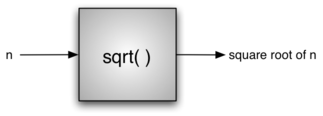
\includegraphics[width=3in]{images/blackbox.png}
\end{figure}
